\section{Results} \label{sec:results}
From the posteriors of galaxy properties inferred using
PROVABGS~(Section~\ref{sec:provabgs}), we derive the marginalized posteriors: 
$p(M_* \given {\bfi X_i})$, the marginalized 1D posterior of $M_*$ for galaxy
$i$.
Using these posteriors, we can estimate the SMF of BGS galaxies using
population inference in a hierarchical Bayesian 
framework~\citep[\emph{e.g.}][]{hogg2010, foreman-mackey2014, baronchelli2020}.
In other words, we infer $p(\phi\given\{{\bfi X_i}\})$, the probability
distribution of population hyperparameters $\phi$ that describe the SMF,
$\Phi(M_*; \phi)$, given the DESI observations, $\{{\bfi X_i}\}$. 
For the SMF, we use a Gaussian Mixture Model~\citep[GMM;][]{press1992, mclachlan2000}, 
which provides a highly flexible parameterization for describing population
distributions: 
\begin{equation}
    \Phi(M_*; \phi) = \sum\limits_{j=1}^{k} \mathcal{N}(M_*; \phi_j).
\end{equation} 
$k$ represents the number of Gaussian components. 
$\phi_j$ represent the mean and standard deviation of the $j^{\rm th}$ Gaussian
component of the GMM. 

We take this approach over the standard approach that use point estimates of
$M_*$ because we can correctly propagate the uncertainties in our $M_*$
measurements and more robustly estimate the $M_*$ distribution --- \emph{ie.}
SMF. 
\cite{malz2020} demonstrated in the context of inferring redshift
distributions from individual photometric redshift measurements that using
point estimates is statistically incorrect and can lead to biased redshift
distributions. 
We emphasize that \cite{malz2020} is an analogous analysis with a similar goal
of measuring a 1D galaxy property distribution. 

To infer $p(\phi\given\{{\bfi X_i}\})$, we follow the same approach described
in \cite{hahn2022}:
\begin{align}\label{eq:popinf}
p(\phi \given \{{\bfi X_i}\}) 
    =&~\frac{p(\phi)~p( \{{\bfi X_i}\} \given \phi)}{p(\{{\bfi X_i}\})}\\
    =&~\frac{p(\phi)}{p(\{{\bfi X_i}\})}\int p(\{{\bfi X_i}\} \given \{\theta_i\})~p(\{\theta_i\} \given \phi)~{\rm d}\{\theta_i\}.\\
    =&~\frac{p(\phi)}{p(\{{\bfi X_i}\})}\prod\limits_{i=1}^N\int p({\bfi X_i} \given \theta_i)~p(\theta_i \given \phi)~{\rm d}\theta_i\\
    =&~\frac{p(\phi)}{p(\{{\bfi X_i}\})}\prod\limits_{i=1}^N\int \frac{p(\theta_i \given {\bfi X_i})~p({\bfi X_i})}{p(\theta_i)}~p(\theta_i \given \phi)~{\rm d}\theta_i\\
    =&~p(\phi)\prod\limits_{i=1}^N\int \frac{p(\theta_i \given {\bfi X_i})~p(\theta_i \given \phi)}{p(\theta_i)}~{\rm d}\theta_i. 
\intertext{
    We estimate the integral using $S_i$ Monte Carlo samples from the
    individual posteriors $p(\theta_i \given {\bfi X_i})$: 
}
    \approx&~p(\phi)\prod\limits_{i=1}^N\frac{1}{S_i}\sum\limits_{j=1}^{S_i}
    \frac{p(\theta_{i,j} \given \phi)}{p(\theta_{i,j})}.
\end{align} 

%BGS provides two samples: BGS Bright and Faint. 
%Galaxies in BGS Bright are selected based on a $r < 19.5$ flux limit, while
%the ones in BGS Faint are selected based on a fiber-magnitude and color limit
%and $r < 20.0175$ flux limit. 
Since the sample of BGS galaxies is not volume-limited and complete as a
function of $M_*$, we must account for the selection effect and incompleteness
when estimating the SMF. 
To account for the selection effects of the BGS samples, we include weights
derived from $z^{\rm max}$, the maximum redshift that galaxy $i$ could be
placed and still be included in the BGS samples. 
We derive $z^{\rm max}_i$ for every galaxy using by redshifting the SED
predicted by the best-fit parameters. 
We then derive $V^{\rm max}_i$, the comoving volume out to $z^{\rm max}_i$, and
include a factor of $1/V^{\rm max}_i$ in the galaxy weight $w_i$. 

Next, we include correction weights for spectroscopic incompleteness driven by
fiber assignment and redshift failures. 
Incompletenss from fiber assignment is due to the fact that DESI is not able to
assign fibers to all galaxies included in the BGS target selection. 
Furthermore, due to galaxy clustering there is significant variation in the
assignment probability. 
Meanwhile, incompleteness from redshift failure is caused by the fact that we
do not successfully measure the redshift for every spectra and the redshift
failure rate depends on the surface brightnesses of the galaxies and the
signal-to-noise ratio of the spectra. 
We describe how we derive $w_{i, {\rm FA}}$ and $w_{i, {\rm ZF}}$, the
incompleteness correction weights for fiber assignment and redshift failures in
Appendix~\ref{sec:spec_comp}. 
Each BGS galaxy is assigned a weight of 
$w_i = (w_{i, {\rm FA}}\times w_{i, {\rm ZF}})/V^{\rm max}_i$.

We modify Eq.~\ref{eq:popinf} to include $w_i$: 
\begin{align}
p(\phi \given \{{\bfi X_i}\}) 
    \approx&~\frac{p(\phi)}{\prod\limits_{i=1}^N p({\bfi X_i})^{w_i}} 
    \prod\limits_{i=1}^N \left(\int p({\bfi X_i} \given \theta_i)~p(\theta_i \given \phi)~{\rm d}\theta_i \right)^{w_i} \\ 
    \approx&~\frac{p(\phi)}{\prod\limits_{i=1}^N p({\bfi X_i})^{w_i}} 
    \prod\limits_{i=1}^N \left( \sum\limits_{j=1}^{S_i}
    \frac{p(\theta_{i,j} \given \phi)}{p(\theta_{i,j})} \right)^{w_i} \\
    \approx&~\frac{p(\phi)}{\prod\limits_{i=1}^N p({\bfi X_i})^{w_i}} 
    \prod\limits_{i=1}^N \left( \sum\limits_{j=1}^{S_i}
    \frac{q_\phi(\theta_{i,j})}{p(\theta_{i,j})} \right)^{w_i}.
\end{align} 

In practice, we do not derive the full posterior 
$p(\phi \given \{{\bfi X_i}\})$. 
Instead we derive the maximum a posteriori (MAP) hyperparameter 
$\phi_{\rm MAP}$ that maximizes $p(\phi \given \{{\bfi X_i}\})$ or 
$\log p(\phi \given \{{\bfi X_i}\})$.
We expand, 
\begin{align}
\log p(\phi \given \{{\bfi X_i}\}) 
    \approx&~\log p(\phi) + % \sum\limits_{i=1}^N w_i \log w_i + 
    \sum\limits_{i=1}^N w_i \log \left(\sum\limits_{j=1}^{S_i} \frac{q_\phi(\theta_{i,j})}{p(\theta_{i,j})} \right).
\end{align} 
Since the first two terms are constant, we derive $\phi_{\rm MAP}$ by
maximizing 
\begin{equation}
    \max_\phi~~\sum\limits_{i=1}^N w_i \log \left(\sum\limits_{j=1}^{S_i} \frac{q_\phi(\theta_{i,j})}{p(\theta_{i,j})} \right).
\end{equation}
using the {\sc Adam} optimizer~\citep{kingma2017}.  
We derive $\phi_{\rm MAP}$ for BGS galaxies in redshift bins of width 
$\Delta z = 0.04$ starting from $z =0.01$. 
This enables us to examine the redshift evolution of the SMF within BGS. 

%\approx&~\log p(\phi) - 
%\log \prod\limits_{i=1}^N p({\bfi X_i})^{w_i} + 
%\log \prod\limits_{i=1}^N \left(\int p({\bfi X_i} \given \theta_i)~p(\theta_i \given \phi)~{\rm d}\theta_i \right)^{w_i} \\
%\approx&~\log p(\phi) - 
%\sum\limits_{i=1}^N w_i \log p({\bfi X_i}) + 
%\sum\limits_{i=1}^N w_i \log \left(\int p({\bfi X_i} \given \theta_i)~p(\theta_i \given \phi)~{\rm d}\theta_i \right) \\
%\approx&~\log p(\phi) + 
%\sum\limits_{i=1}^N w_i \log \left(\frac{1}{w_i} \sum\limits_{j=1}^{S_i} w_{i,j} \frac{p(\theta_{i,j} \given \phi)}{p(\theta_{i,j}} \right) \\

%\subsection{Targeting Completeness} \label{sec:ts}
% https://desi.lbl.gov/trac/wiki/ClusteringWG/LSScat/SV3/version2.1/fulldat
% https://desi.lbl.gov/trac/wiki/ClusteringWG/LSScat/SV3/version2.1/fullran

\begin{figure}
\begin{center}
    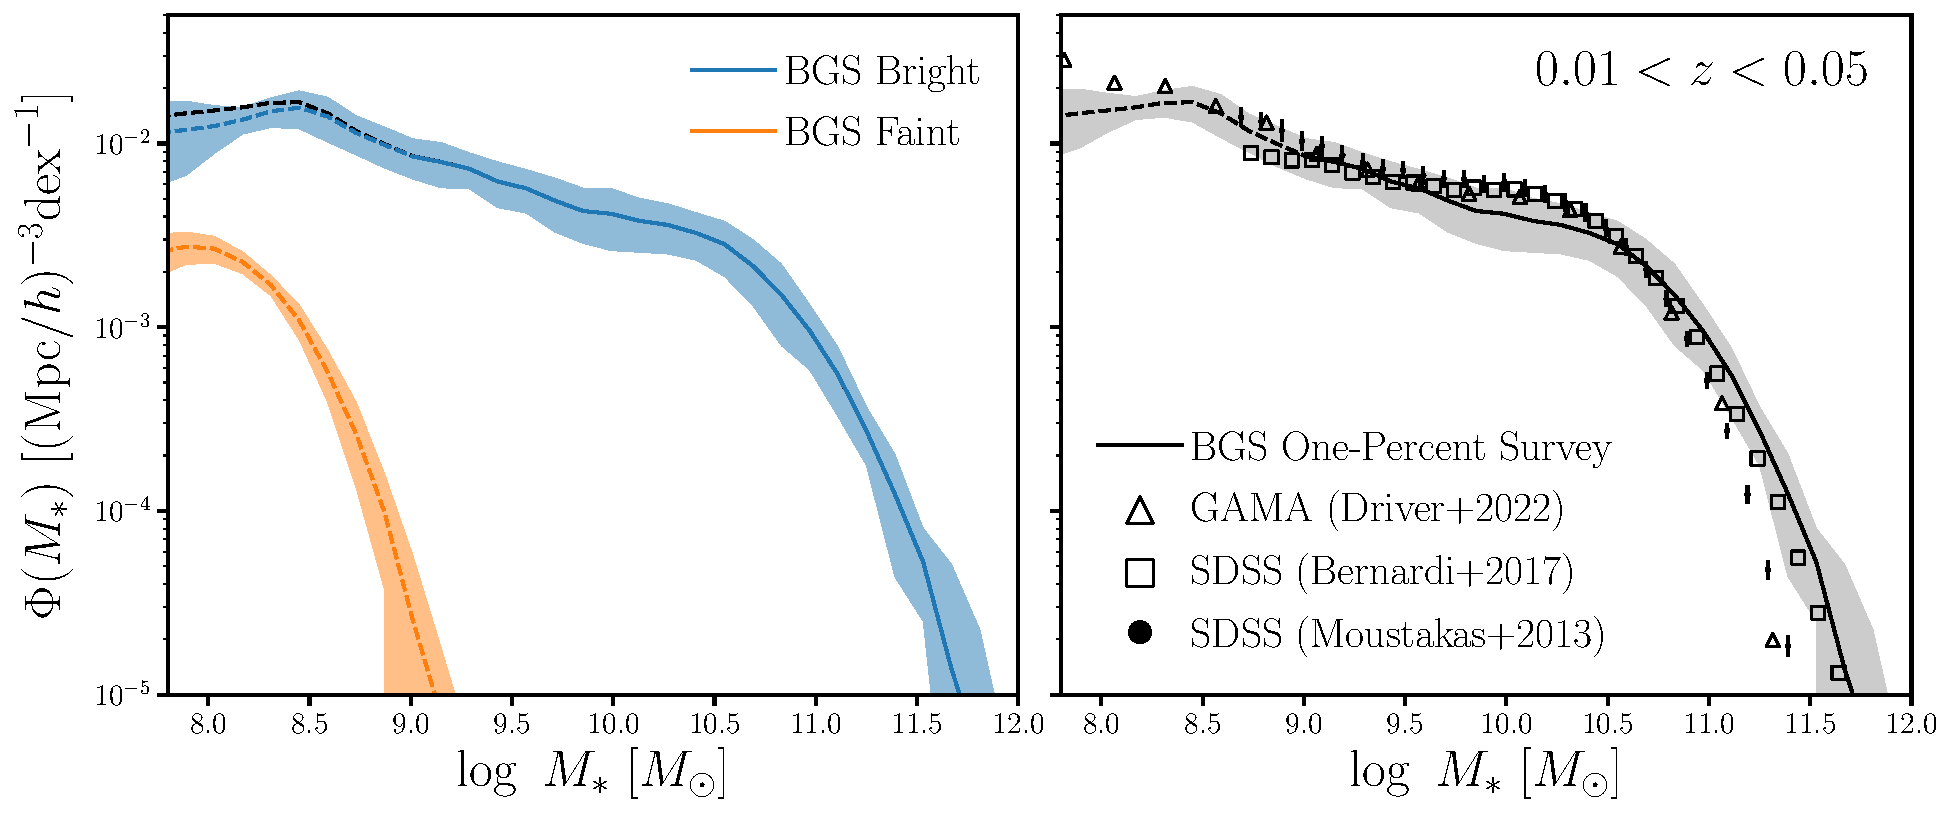
\includegraphics[width=0.9\textwidth]{figs/psmf_bgs_any_comp.pdf} 
    \caption{
        The probabilistic SMF (pSMF) of BGS galaxies in the One-Percent Survey
        at $0.01 < z < 0.05$ (black line). 
        We represent uncertainties on the pSMF, estimated using a standard
        jackknife technique (Appendix~\ref{sec:jack}), in the shaded regions.
        The solid line represents the pSMF above the completeness limit 
        $M_* > M_{\rm lim} = 10^{8.975}M_\odot$ (Appendix~\ref{sec:mscomp}).
        In the left panel, we present the pSMFs of BGS Bright (blue) and
        Faint (orange) galaxies. 
        In the right panel, we include SMF measurements from previous
        spectroscopic surveys for comparison: SDSS~\citep{moustakas2013,
        bernardi2017} and GAMA~\citep{driver2022}. 
        Overall, the pSMF of BGS are in good agreement with SMF
        measurements from previous surveys.  
    }\label{fig:psmf}
\end{center}
\end{figure}

\begin{figure}
\begin{center}
    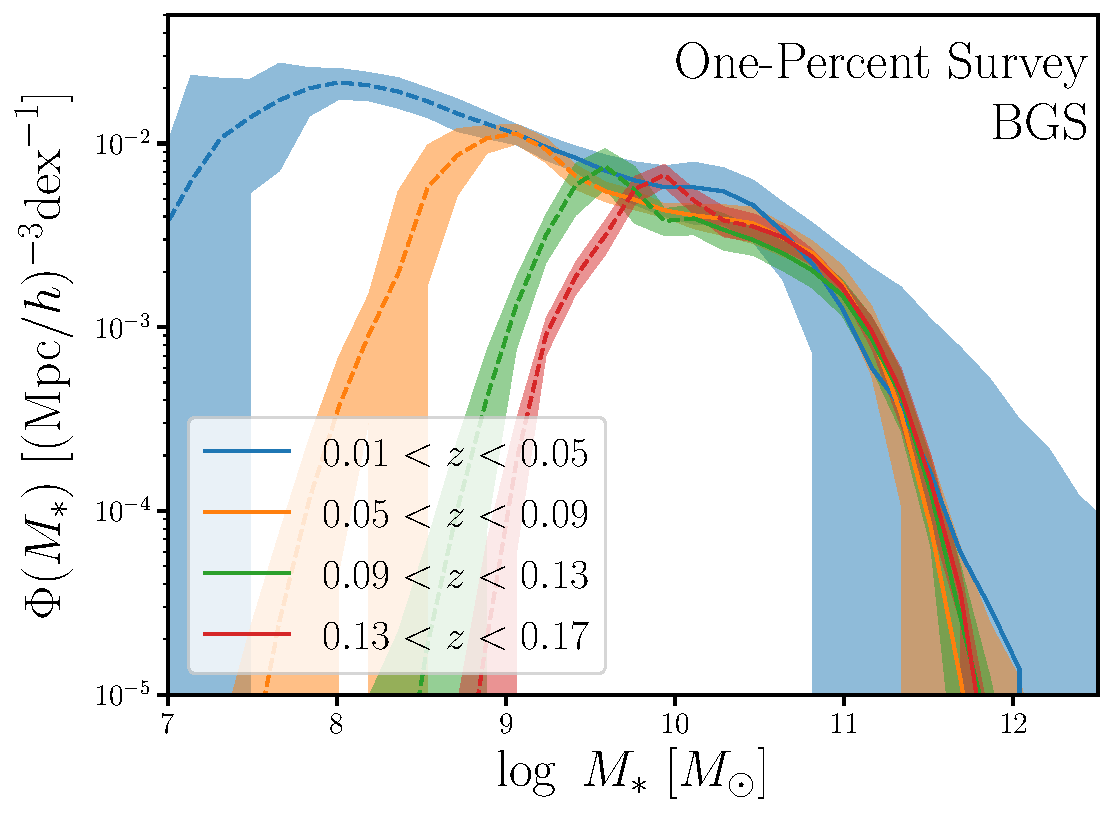
\includegraphics[width=0.5\textwidth]{figs/psmf_bgs_any_zevo.pdf} 
    \caption{
        The BGS pSMF over the redshift range $0.01 < z < 0.17$ in bins of
        $\Delta z = 0.04$. 
        The shaded regions represent the uncertainties on the pSMF, estimated
        using a standard jackknife technique.
        The solid lines represent the pSMF above the completeness limit 
        $M_* > M_{\rm lim}$ while the dashed lines represent the pSMF below
        the limit.
        There is no significant redshift evolution of the pSMF given their
        statistical uncertainties. 
        The main BGS survey will observe $>100\times$ more galaxies than the
        One-Precent Survey. 
    }\label{fig:psmfz}
\end{center}
\end{figure}

\subsection{The Probabilistic Stellar Mass Function} \label{sec:psmf}
We present the probabilistic SMF (pSMF) of $0.01 < z < 0.05$ BGS galaxies in the
One-Percent Survey in Figure~\ref{fig:psmf} (black line). 
The shaded regions represent the uncertainties of the pSMF from sample variance,
which we derive using a standard jackknife technique
(Appendix~\ref{sec:uncert}) and are conservative estimates~\citep{norberg2009}. 
In the left panel, we also present the pSMFs of the BGS Bright (blue) and Faint
(orange) galaxies.  
BGS Bright galaxies are selected primarily using a $r > 19.5$ magnitude limit. 
As a result, the BGS Bright sample is $M_*$ complete above $M_{\rm lim} >
10^{8.975}M_\odot$. 
We derive $M_{\rm lim}$ in Appendix~\ref{sec:mscomp} and mark the pSMF above
the completeness limit in solid and below the limit in dashed. 
Meanwhile, the BGS Faint sample is selected using a surface brightness and
color selection.   
It includes fainter galaxies, $19.5 < r < 20.175$, with overall lower $M_*$
than the BGS Bright sample. 

In the right panel, we compare the BGS pSMF to SMF measurements from previous 
spectroscopic surveys: SDSS~\citep{moustakas2013, bernardi2017} (black circle
and square) and GAMA~\citep{driver2022} (black triangle).
For the \cite{driver2022} SMF, we include a 0.0807 dex correction that the
authors recommend to re-normalize the SMF and correction to $z=0$. 
We note that there is significant variance in SMF measurements in the
literature, especially at the high $M_*$ end. 
This is partly due to the different modeling methodologies used to derive
$M_*$, which can contribute >0.1 dex discrepancies~\citep{pacifici2023}. 
Furthermore, there are also discrepancies due to photometric corrections
applied to SDSS photometry, assumptions on the stellar populations, and
dust~\citep{bernardi2017}.
We reserve a more detailed comparison of BGS $M_*$ measurements using different
methods for future work. 
Overall, we find good agreement with previous SMF measurements, especially in
the intermediate $M_*$ range where we precisely infer the pSMF.  

In Figure~\ref{fig:psmfz}, we present the redshift evolution of the pSMF from
$z\sim 0.15$ to 0.03 in redshift bins of $\Delta z = 0.04$. 
The shaded region represent the jackknife uncertainties for the pSMF.
The solid line represents the pSMF above $M_{\rm lim}$ while the dashed lines
represent the pSMF below the limit. 
We only include 4 redshift bins, since $M_{\rm lim} > 10^{10.5}M_\odot$ for 
$z > 0.17$ (Table~\ref{tab:mscomp}).
The pSMFs in Figure~\ref{fig:psmfz} do not reveal a significant redshift
dependence given their uncertainties. 
We note that the large uncertainties for the $0.01 < z < 0.05$ pSMF is driven
by large-scale structure at RA $\sim 195$ deg, Dec $\sim 28$ deg, and 
$z\sim0.244$. 
However, we emphasize that the main BGS survey will observe $>100\times$ the
number of BGS galaxies in the One-Percent Survey and enable pSMF measurements
with unprecedented precision. 

\begin{figure}
\begin{center}
    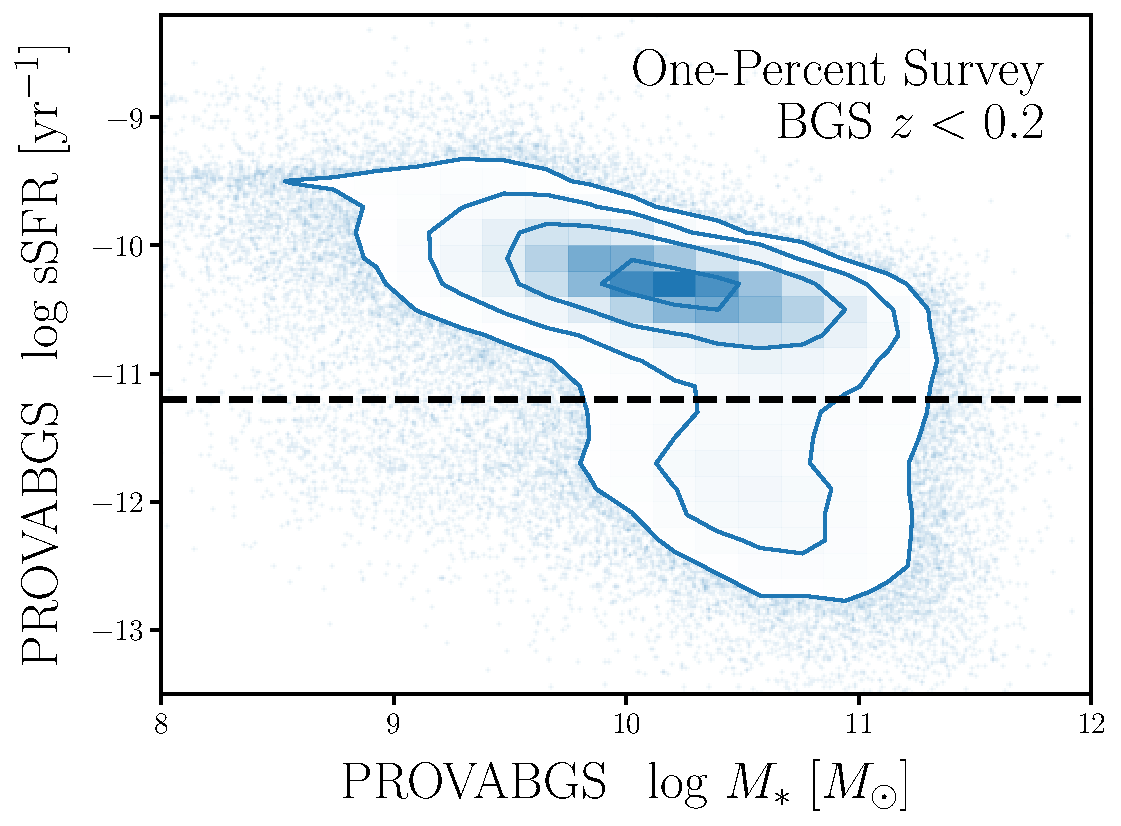
\includegraphics[width=0.5\textwidth]{figs/sfq.pdf} 
    \caption{
        The $M_*-{\rm sSFR}$ distribution of BGS galaxies at $z < 0.2$. 
        sSFR is derived using $\overline{\rm SFR}$, average SFR over the last 1
        Gyr, inferred using PROVABGS. 
        The $M_*-{\rm sSFR}$ distribution is bimodal with star-forming galaxies
        lying on the star-forming sequence.
        We classify galaxies with ${\rm sSFR} > 10^{-11.2}\,{\rm yr}^{-1}$ as
        star-forming galaxies and ${\rm sSFR} < 10^{-11.2}\,{\rm yr}^{-1}$ as
        quiescent. 
    }\label{fig:sfq}
\end{center}
\end{figure}


\begin{figure}
\begin{center}
    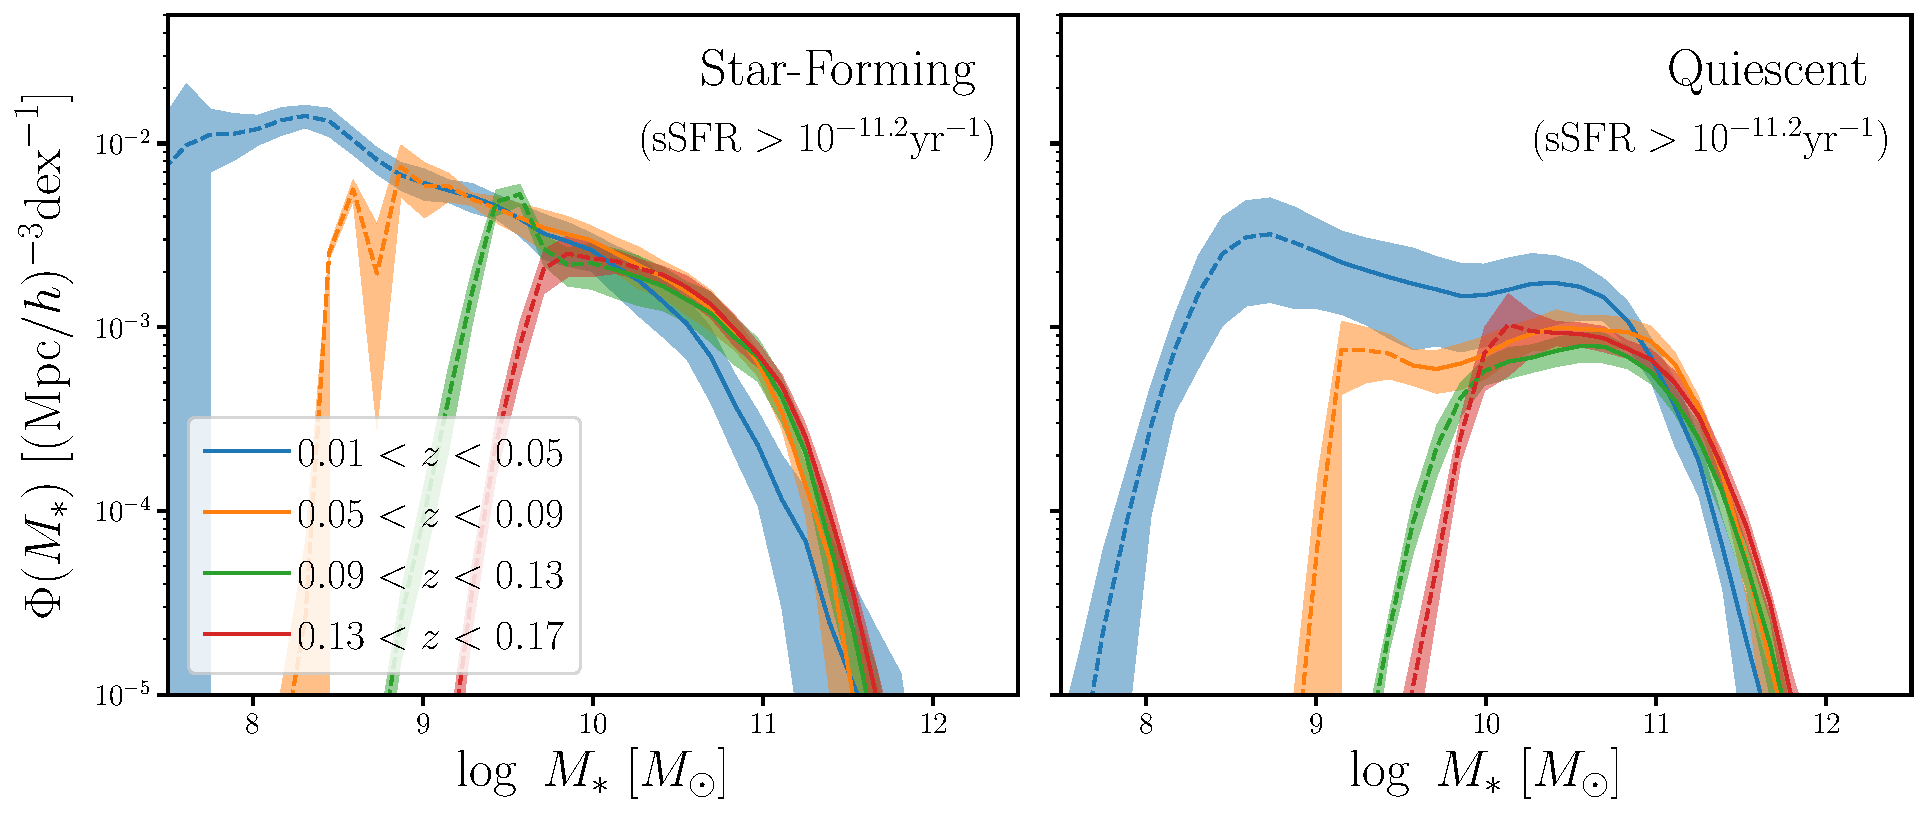
\includegraphics[width=0.9\textwidth]{figs/psmf_bgs_bright_sfq.pdf} 
    \caption{
        The pSMF of star-forming (left) and quiescent (right) BGS Bright
        galaxies over $0.01 < z < 0.17$ in bins of $\Delta z = 0.04$. 
        Star-forming and quiescent galaxies are classified using an empirically
        determined ${\rm sSFR} = 10^{-11.2}{\rm yr}^{-1}$ cut. 
        We represent the uncertainties for the pSMF in the shaded regions and 
        the pSMFs above/below the $M_*$ completeness limits in solid/dashed
        lines.
        At $M_* < 10^{11}M_\odot$ we find an increase in the quiescent galaxy
        population with no significant evolution of the star-forming population.
    }\label{fig:sfqsmf}
\end{center}
\end{figure}


\begin{figure}
\begin{center}
    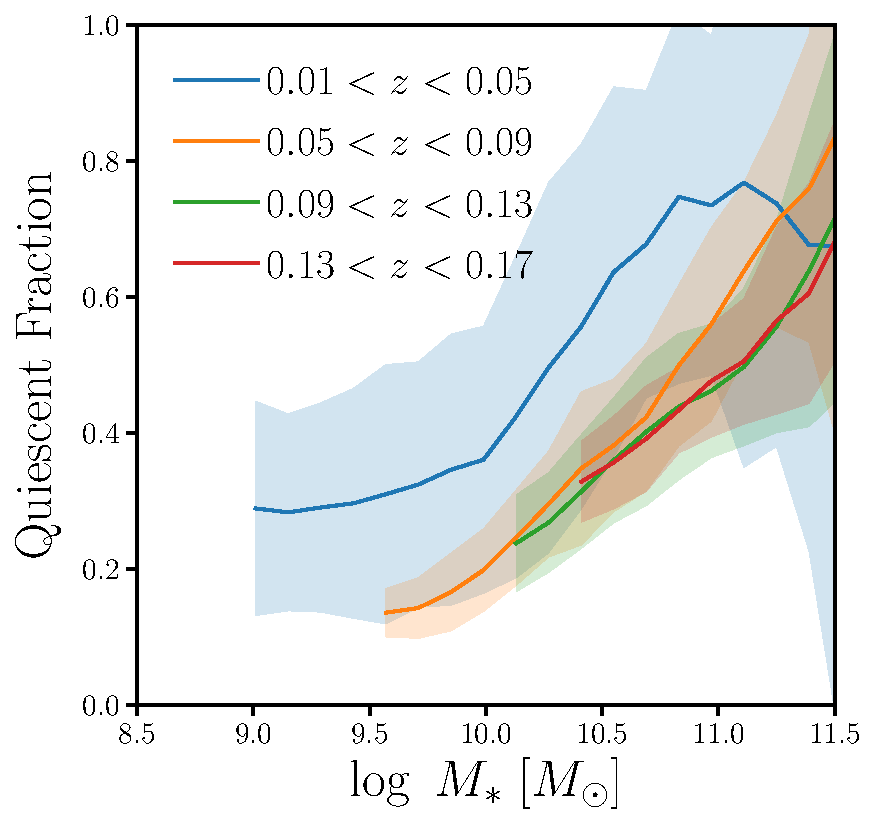
\includegraphics[width=0.45\textwidth]{figs/qf_bgs_bright.pdf} 
    \caption{
        The quiescent fraction of BGS Bright galaxies over $0.01 < z < 0.17$ in
        bins of $\Delta z =0.04$.
        We present the uncertainties in the shaded region and only include  
        the quiescent fraction above the $M_*$ completeness limit. 
        The quiescent fractions increase with $M_*$ to $\sim$1 at
        $M_*\sim10^{11.5}M_\odot$. 
        The quiescent fractions also suggest an increase in the quiescent
        population with lower redshift at low $M_*$.
    }\label{fig:qf}
\end{center}
\end{figure}

\subsection{Star-Forming and Quiescent Galaxies in the BGS} \label{sec:sfq}
In addition to the pSMF of the full galaxy population, PROVABGS also infers
$\overline{\rm SFR}$, average SFR over the last 1 Gyr, so we can examine the
pSMF of the star-forming and quiescent subpopulations. 
In Figure~\ref{fig:sfq}, we present the distribution of $M_*$ versus specific
SFR, ${\rm sSFR} = \overline{\rm SFR}/M_*$, for BGS Bright (blue) and Faint
(orange) galaxies at $z < 0.2$. 
BGS galaxies form a bimodal $M_*-{\rm sSFR}$ distribution, with star-forming
galaxies lying on the so-called ``star-forming
sequence''~\citep[SFS;][]{noeske2007, daddi2007, salim2007, speagle2014,
hahn2019} and quiescent galaxies lying $\gtrsim$1 dex below the sequence. 
BGS Faint galaxies have lower $M_*$ than BGS Bright galaxies and are primarily
star-forming galaxies. 
This is consistent with the fact that the $(z - W1)-1.2(g-r)+1.2$ color used to
select BGS Faint galaxies is a proxy for H$\alpha$ and H$\beta$ emission lines.  
To further examine the star-forming and quiescent galaxy populations, we
classify BGS Bright galaxies as star-forming or quiescent using a 
${\rm sSFR} = 10^{-11.2}\,{\rm yr}^{-1}$ cut. 
We determine this cut empirically based roughly on the sSFR of the ``green
valley'' between the SFS and the quiescent mode. 
We opt for a sSFR cut rather than more sophisticated methods in the
literature~\citep[\emph{e.g.}][]{hahn2019, donnari2019} for simplicity. 
In Figure~\ref{fig:sfqsmf}, we present the pSMF of star-forming and quiescent
BGS Bright galaxies at $0.01 < z < 0.17$ in bins of $\Delta z = 0.04$.
The shaded regions represent the jackknife uncertainties for the pSMF. 
The solid lines represent the pSMFs above the completeness limit while the
dashed lines represent the pSMFs below the limit. 
The pSMF of quiescent galaxies suggest an increase in the number of galaxies
below $M_* < 10^{11}M_\odot$.
Meanwhile, the pSMF of star-forming galaxies shows no significant evolution
over $0.01 < z < 0.17$. 

Next, we present the fraction of quiescent galaxies as a function of $M_*$ over
$0.01 < z < 0.17$ in Figure~\ref{fig:qf}.
The quiescent fraction is derived by taking the ratio of the pSMFs of quiescent
galaxies over all galaxies in BGS Bright and measured for each $\Delta z =0.04$
bin.
The shaded region represent the uncertainties derived from propagating the
jackknife uncertainties of the pSMFs. 
We only include the quiescent fraction above the $M_*$ completeness limit: $M_*
> M_{\rm lim}$. 
Overall, the quiescent fraction increases with $M_*$ to 1 at
$M_*\sim10^{11.5}M_\odot$. 
The quiescent fraction also suggests an increase in the quiescent population
with redshift at low $M_*$. 
However, there is no clear trend given the statistical uncertainties.
Upcoming observations from the main operations of the BGS will increase the
number of BGS galaxies by >100$\times$ and dramatically improve the precision
of quiescent fraction measurements. 
